\documentclass[9pt,a4paper]{extarticle}
\usepackage[a4paper,margin=1.55cm]{geometry}
\usepackage[utf8]{inputenc}
\usepackage[T1]{fontenc}
\usepackage{helvet}
\renewcommand{\familydefault}{\sfdefault}
\DeclareUnicodeCharacter{00D7}{\ensuremath{\times}}
\DeclareUnicodeCharacter{2013}{\textendash}
\DeclareUnicodeCharacter{201C}{``}
\DeclareUnicodeCharacter{201D}{''}
\DeclareUnicodeCharacter{2192}{\ensuremath{\rightarrow}}
\usepackage{graphicx}
\usepackage{enumitem}
\usepackage{ragged2e}
\usepackage{microtype}
\usepackage{parskip}
\setlength{\parindent}{0pt}
\setlength{\parskip}{4pt}
\pagestyle{empty}
\setlist[itemize]{leftmargin=1.5em,itemsep=1.2pt,topsep=2pt,parsep=0pt,partopsep=0pt,label=\textbullet}
\newcommand{\Sec}[1]{\vspace{2pt}\noindent\textbf{#1}\par\vspace{2pt}}
\newcommand{\Sub}[1]{\vspace{2pt}\noindent\textbf{#1}\par\vspace{1pt}}
\begin{document}
\fontsize{8.6}{10.2}\selectfont

Faculty of Electrical Engineering – University of Sarajevo\\
Course: Artificial Intelligence\\
Professor: Izudin Džafić\\
Team: Rijalda Šaćirbegović, Almir Mustafić, Tarik Bajrović

\vfill
\begin{center}
{\fontsize{17}{20}\selectfont\textbf{PatternScope AI}}\\[8pt]
{\fontsize{12}{15}\selectfont\textbf{Hybrid Pattern Recognition System}}
\end{center}
\vfill
\newpage

\Sec{Executive Summary}
PatternScope AI is a hybrid pattern recognition system that supports the digitization of handwritten academic material. The current implementation recognizes handwritten digits, geometric shapes, and custom symbols. Users can upload images. The system returns per-model predictions, confidence scores, and an ensemble result. Users can also provide corrections during runtime.

The project focuses on the first part of a larger workflow. Students, teaching assistants, and professors often prepare notes, exam materials, lab reports, formulas, and diagrams by hand. Converting these materials into digital form takes time and may require several software tools. The project uses pattern recognition as the first step toward converting this material into reusable digital content.

The planned platform will assemble recognized elements into text, equations, and vector drawings. It will export content to editable PDF and LaTeX formats. The project proposes hosting the platform at the University of Sarajevo. Students, teaching assistants, and professors at Bosnian universities would use the platform without subscription fees. The hosting model would keep academic material on local university servers rather than third-party clouds.

\Sec{1. About the Project}
PatternScope AI currently performs three recognition tasks.
\begin{itemize}
\item The system recognizes handwritten digits from 0 to 9.
\item The system recognizes circles, squares, and triangles.
\item The system recognizes checkmarks, crosses, and hearts.
\end{itemize}
Users can upload images. The system returns predictions, confidence scores, and model comparisons. When users provide the correct label, the system updates its internal models during runtime.

The next phase will use the same recognition engine as a base for the following functions.
\begin{itemize}
\item The platform will assemble recognized elements into text.
\item The platform will assemble recognized elements into equations.
\item The platform will assemble recognized elements into vector drawings.
\item The platform will export content to editable PDF and LaTeX formats.
\end{itemize}
\newpage

\Sec{2. System Architecture Overview}
PatternScope AI is built as a modular hybrid AI engine composed of:
\begin{itemize}
\item Data processing pipeline
\item Multiple supervised learning models
\item An ensemble decision mechanism
\item A rule-based fallback system
\item Real-time active learning agent
\item GUI interface via natID framework
\end{itemize}
The backend logic is implemented in C++14 and exposed to the GUI through a central Engine class.

\Sec{3. Technology Stack}
The system is implemented using:
\begin{itemize}
\item C++14 – Core AI engine and model implementation
\item CMake – Cross-platform build management
\item stb\_image – Image loading and preprocessing
\item natID GUI framework – Interactive desktop interface
\end{itemize}
The system is fully offline and cross-platform compatible.

\Sec{4. Datasets}
The system is trained on three datasets:

\Sub{4.1 MNIST Dataset}
\begin{itemize}
\item 60,000 training images
\item 10,000 test images
\item 28×28 grayscale digit images
\item IDX file format
\end{itemize}

\Sub{4.2 Quick Draw Shapes Dataset}
\begin{itemize}
\item 1,000 training samples per class
\item 200 test samples per class
\item Classes: circle, square, triangle
\end{itemize}

\Sub{4.3 Quick Draw Symbols Dataset}
\begin{itemize}
\item 1,000 training samples per class
\item 200 test samples per class
\item Classes: checkmark, cross, heart
\end{itemize}
\newpage

All images are:
\begin{itemize}
\item Resized to 28×28
\item Normalized to [0, 1]
\item Converted into feature vectors
\end{itemize}
Training is performed using a standard train-test split.

\Sec{5. Algorithms \& Models}
PatternScope AI uses a hybrid ensemble composed of five components:
\begin{itemize}
\item K-Nearest Neighbors (KNN)
\item Naive Bayes
\item Mini Multi-Layer Perceptron (MLP)
\item A* Template Matcher
\item Rule-Based Engine (Fallback)
\end{itemize}
Each model contributes unique strengths in classification, explainability, and robustness.

\Sec{6. How the Algorithms Work}
\Sub{6.1 K-Nearest Neighbors (KNN)}
KNN stores all training feature vectors.

During prediction:

Euclidean distance is computed between input and stored samples.

The 3 nearest neighbors are selected.

The most frequent label among neighbors is returned.

Confidence is computed based on neighbor agreement and distance.

Strength:

Immediate adaptability through active learning.

No parameter retraining required.

\Sub{6.2 Naive Bayes}
Naive Bayes models each pixel using a Gaussian distribution.

During training:
\newpage

Mean and variance are computed per pixel per class.

During prediction:

Class likelihood is computed using Gaussian probability.

The class with maximum posterior probability is selected.

Strength:

Fast probabilistic inference.

Works well with grayscale intensity distributions.

\Sub{6.3 Mini Multi-Layer Perceptron (MLP)}
Architecture:
\begin{itemize}
\item 784 input neurons (28×28 pixels)
\item 64 hidden neurons
\item Output neurons depend on task (10 for digits, 3 for shapes/symbols)
\end{itemize}
Training:
\begin{itemize}
\item Random weight initialization (-0.5 to 0.5)
\item 5 epochs
\item Learning rate: 0.01
\item Backpropagation for gradient updates
\end{itemize}
Strength:
\begin{itemize}
\item Captures nonlinear pixel relationships.
\item Higher accuracy for complex patterns.
\end{itemize}

\Sub{6.4 A* Template Matcher}
Uses first 200 training samples as templates.

Prediction process:
\begin{itemize}
\item Compute Euclidean distance to each template.
\item Use priority queue for sorting.
\item Return closest match.
\end{itemize}
Strength:

Deterministic
\newpage

Fully explainable

Allows template visualization

Unlike neural networks, A* provides transparent reasoning.

\Sub{6.5 Rule-Based Engine}
Triggered when ensemble confidence $<$ 0.4.

Uses structural features:
\begin{itemize}
\item Edge count
\item Corner count
\item Aspect ratio
\item Symmetry
\end{itemize}
Applies deterministic rules such as:

“4 corners + rectangular geometry → likely 0 or 8”

Purpose:
\begin{itemize}
\item Prevent silent failures
\item Ensure fallback decision path
\end{itemize}

\Sec{7. Ensemble Decision Mechanism}
Each model returns:

Predicted label

Confidence score

Confidence aggregation

Scores per label are summed

Highest total score wins

Final confidence = total\_score / 4.0

If final confidence $<$ 0.4:

→ Rule-Based Engine overrides decision.

This ensures:

Robust decision-making
\newpage

Honest uncertainty handling

Multi-model agreement verification

\Sec{8. Active Learning Mechanism}
When user provides correct label:
\begin{itemize}
\item KNN appends new feature vector
\item Naive Bayes updates mean \& variance incrementally
\item MLP performs one forward + backward update
\end{itemize}
These updates occur in RAM during runtime.

This enables:
\begin{itemize}
\item Incremental adaptation
\item Institution-specific handwriting learning
\item Continuous system improvement
\end{itemize}

\Sec{9. Model Training \& Serialization}
Training is performed offline using:

./trainer

After training:

Models are serialized into:
\begin{itemize}
\item knn.txt
\item nb.txt
\item mlp.txt
\item astar.txt
\end{itemize}
At runtime:

Models are loaded into memory

No retraining required

This reduces startup latency and ensures deployment efficiency.

\Sec{10. Graphical User Interface (PatternVision++)}
The natID-based GUI allows:
\begin{itemize}
\item Mode selection (Digits, Shapes, Symbols)
\end{itemize}
\newpage

Image upload

Real-time predictions

Model comparison panel

Confidence visualization

Active learning feedback

Confusion matrix \& metrics view

\vspace{6pt}
\begin{center}
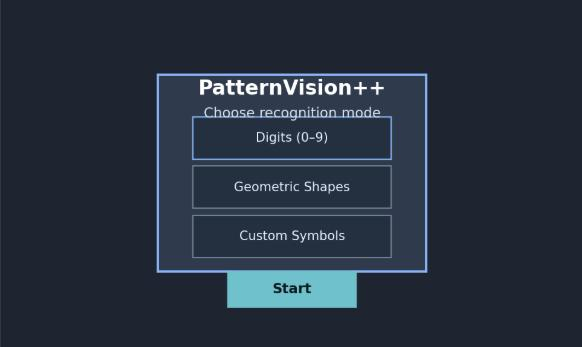
\includegraphics[width=0.64\textwidth]{assets/ps-000.jpg}\\[4pt]
Caption: Figure 1 – PatternVision++ Mode Selection Interface

\vspace{10pt}
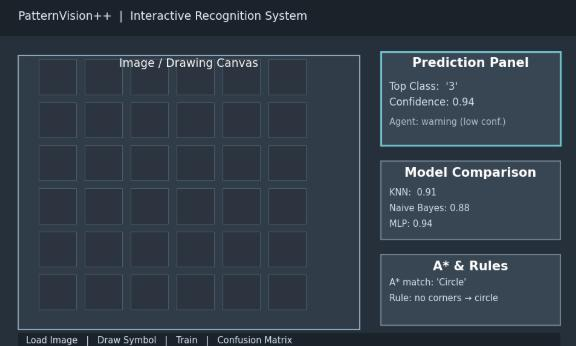
\includegraphics[width=0.64\textwidth]{assets/ps-001.jpg}\\[4pt]
Caption: Figure 2 – Live Prediction and Model Comparison Panel
\end{center}
\newpage

\Sec{11. Problem and Market Gap}
Every semester, students and staff create exam materials, lab reports, notes, formulas, diagrams, and geometric drawings by hand. Converting this material into digital form takes time. Using several software tools can shift attention from course content to software use. Paper-based notes are also difficult to reuse across new groups of students.

The team reviewed existing tools while defining the project. Microsoft 365 and Mathpix use recurring subscription models. Apple Math Notes offers a free option but requires Apple devices. The project therefore targets a gap for a device-independent academic platform that can be used across Bosnian universities.

\Sec{12. Target Users}
\begin{itemize}
\item Students can digitize notes, equations, and study materials.
\item Teaching assistants can digitize exercises, diagrams, and lab materials.
\item Professors can convert handwritten course material into editable content.
\item Universities can store and reuse academic material across courses and student generations.
\end{itemize}

\Sec{13. Roadmap and Hosting}
The current phase recognizes individual digits, shapes, and symbols. The next phase will assemble recognized elements into text, equations, and vector drawings. The platform will export content to editable PDF and LaTeX formats.

The project proposes hosting the platform at the University of Sarajevo. Students, teaching assistants, and professors at Bosnian universities would use the platform without subscription fees. The hosting model would keep academic work and research notes on local university servers rather than third-party clouds.

\end{document}
